\documentclass{article}
\usepackage[utf8]{inputenc}
\usepackage{Mic}
\geometry
{
 a4paper,
 total={170mm,257mm},
 left=20mm,
 top=20mm,
}

\title{\Bigg01.020 Design Thinking Project III (MU) \\ Towards Zero Hunger: \\ A Cross-Country Analysis of Factors Affecting Food Insecurity}

\author{Cohort 08 Group 04}

\date{\today}

\begin{document}

\maketitle
\thispagestyle{empty}

\begin{center}
\begin{tabular}{ |c|c|c|c| } 
 \hline
  ID & Name & ID & Name \\
 \hline
  1006617 & Michael Hoon Yong Hau & 1006954 & Joshua John Lee Shi Kai \\
 \hline
  1006651 & Wong Qi Yuan Kenneth & 1007085 & Yaromir Viswanathan \\
 \hline
\end{tabular}
\end{center} 

%\section*{Contributions}

%\begin{itemize}
%    \item Michael Hoon Yong Hau:
%    \item Joshua John Lee Shi Kai:
%    \item Wong Qi Yuan Kenneth:
%    \item Yaromir Viswanathan: 
%\end{itemize}

\tableofcontents
\thispagestyle{empty}

\newpage
\setcounter{page}{1}

\section{Introduction} 
The world faces an unprecedented challenge — to feed a projected population of 9 billion by 2050 while ensuring safe, sustainable, and equitable food systems \cite{doi:10.1126/science.1185383}. This imperative is not only a matter of meeting the demands of a growing population but is deeply rooted in the fundamental right of every individual to access safe, nutritious, and sufficient food, as underscored by the United Nations (UN) Sustainable Development Goal 2: Zero Hunger \cite{unsdg2}. \\

\noindent In light of this, our project aims to conduct a rigorous cross-country analysis, investigating the intricate factors that influence food insecurity on a global scale. Our problem statement is as follows: 

\begin{formal}
    "How might we identify the \textbf{key factors of influence for food insecurity index} across countries, to facilitate informed and targeted governmental policy interventions?"
\end{formal}

\noindent As such, our main target audience for this project is governmental organisations involved in policy-making for their country's food security. This ensures relevant insights to formulate effective policies and interventions, addressing food security issues based on specific socioeconomic indicators.

\section{Data Collection and Wrangling}
Most of our raw data is obtained from reputable sources such as the Food and Agricultural Organisation of the United Nations \href{https://www.fao.org/home/en}{(FAO)} and the \href{https://data.worldbank.org}{World Bank Group}. Since our data for each variable is sourced from multiple sources (for the year 2022), we have compiled everything into a single sheet as the input for our model. 

\subsection{Data Cleaning}\label{NormalisationImputation}
To prepare the raw datasets into cleaned, usable information, we applied several data cleaning techniques, such as normalisation and imputation. For normalisation in Excel, we used the built-in \verb|=STANDARDISE()| function, which applies z-score normalisation on each row value. As for data imputation, we applied an (Iterative) Multiple-Imputation (MI) technique \cite{MeanImputation} \cite{scikit-learn} to replace the missing data values in our dataset, instead of merely dropping the rows. As for the variables (Gini Index \& Average Temperature) which are not available for the year $2022$, we have imputed using the most recent data. The final dataset can be found in the Excel sheet.

\subsection{Data Transformation}
Furthermore, we have log-transformed GDPpc (Gross Domestic Product per capita) and Minimum Wage, as from the scatter plots obtained of all the predictor variables, they appear to follow a logarithmic trend, shown in Figure \ref{fig:scattergdppc} and Figure \ref{fig:scatterminwage}.

\section{Multiple Linear Regression Model}

Our Multiple Linear Regression Equation is as follows: 

\begin{equation}
    \begin{aligned}
        \mathbf{FII} &= \beta_0 + \beta_1\mathbf{AgriculturalLand(\%)} + \beta_2\mathbf{CO_2Emissions} + \beta_3\mathbf{CPI} + \beta_4\mathbf{GDP} + \beta_5\mathbf{Population} \\ & + \beta_6\mathbf{InfantMortality} + \beta_7\ln{[\mathbf{MinimumWage}]} + \beta_8\mathbf{UnemploymentRate} \\ & + \beta_9\mathbf{LabourForceParticipation(\%)} + \beta_{10}\mathbf{Temperature} + \beta_{11}\mathbf{IdealTemperature} \\ & + \beta_{12}\mathbf{PrecipitationDepth} + \beta_{13}\mathbf{GiniIndex} + \beta_{14}\ln{[\mathbf{GDPpc}]} + \beta_{15}\mathbf{HDI}
    \end{aligned}
\end{equation}

\noindent where \textbf{FII} is the Prevalence of Moderate and Severe Food Insecurity, \textbf{CPI} is the Consumer Price Index, and \textbf{HDI} is the Human Development Index.

\subsection{OLS Parameter Estimates}
Parameter estimates of our original model are given in Table \ref{table: descriptivestatsoriginal}, Appendix \ref{AppB}. Significance levels are indicated with stars below the table. 

\subsubsection{Individual Statistical Significance}\label{IndividualSignificance}
From the \textit{p-values} obtained in Table \ref{table: descriptivestatsoriginal}, we conclude that \textbf{$\bm{\text{CO}_2}$ Emissions}, \textbf{GDP}, \textbf{Population}, \textbf{Infant Mortality}, \textbf{Gini Index}, and \textbf{HDI} are all statistically significant at the 95\% level. 

\subsection{Significance Test for Equation}\label{sec:sigtest}
In order to test the significance of our model, we employ an F-test \cite{Greene2003Econometric}. The null hypothesis of the F-test is given by:

\begin{equation}
    H_0: \bm{\beta_0} = \bm{\beta_1} = \bm{\beta_2} = \bm{\beta_3} = \bm{\beta_4} = \dots = \bm{\beta_{15}} = 0
\end{equation}

\noindent and the F-statistic is 

\begin{equation}\label{eqn:F-stat}
    F = \frac{\mathbf{Mean \; Square \; Regression}}{\mathbf{Mean \; Square \;  Error}} = \frac{{\sum_{i=1}^N (\hat{Y}_i - \hat{Y})^2} / k}{\sum_{i=1}^N (Y_i- \hat{Y})^2/(n-k-1)} = 104.749
\end{equation}

\noindent The calculated F-statistic is $\bm{F = 104.749}$. At the 95\% significance level, the critical value obtained from the F-distribution table on 15 and 179 degrees of freedom is $\bm{F = 2.04}$. Since the F-statistic $\bm{F = 104.749 > 2.04}$, then we can say that there is \textbf{sufficient evidence to reject the null hypothesis at the 95\% significance level}, and \textbf{the equation is statistically significant.} However with this model, there is a high probability that over-fitting has occurred, and there are many variables which are not individually significant. 

\section{Model Improvements}
With the above shortcomings of our model, we suggest several improvement techniques:

\subsection{Feature Engineering}\label{sec: feateng}
We have built a subset model via feature engineering, to separate the original model into an economic model in Equation \ref{economicmodel} (with Economic factors) and a geographical model (with geographical-related factors) in Equation \ref{geographicmodel}. These variables are separated for a better comparison between the significance of economic and geographical factors affecting FII, allowing us to select the best variables for our final model. Parameter estimates of each model is given in Table \ref{table: descriptivestatseconomic} and Table \ref{table: descriptivestatsgeographic}, Appendix \ref{AppB}.

\subsubsection{Economic Model}

\begin{equation}\label{economicmodel}
    \begin{aligned}
        \mathbf{FII} = \beta_0 &+ \beta_1\mathbf{CPI} + \beta_2\ln{[\mathbf{MinimumWage}]} + \beta_3\mathbf{Unemployment} + \beta_4\mathbf{LabourForceParticipation} \\ &+ \beta_5\mathbf{GiniIndex} + \beta_6\mathbf{GDP}
    \end{aligned}
\end{equation}

\subsubsection{Geographic Model}

\begin{equation}\label{geographicmodel}
    \begin{aligned}
        \mathbf{FII} = \beta_0 &+ \beta_1\mathbf{AgriculturalLand(\%)} + \beta_2\mathbf{CO_2Emissions} + \beta_3\mathbf{Population} + \beta_4\mathbf{InfantMortality} \\ &+ \beta_5\mathbf{IdealTemperature} + \beta_6\mathbf{PrecipitationDepth} + \beta_7\mathbf{HDI}
    \end{aligned}
\end{equation}

\subsection{Statistical Significance}\label{sec: statsig}
To determine the variables significant for our final model, we included variables which are statistically significant in both the original model and feature-engineered models (with reference to Tables \ref{table: descriptivestatsoriginal}, \ref{table: descriptivestatseconomic}, \ref{table: descriptivestatsgeographic}, Appendix \ref{AppB}). Furthermore, we have made an exception for \textbf{$\bm{\ln{[\text{MinimumWage}]}}$}, as despite not being statistically significant in the original model, it has the highest t-statistic value (lowest p-value) in the economic model, which prompted us to include it in the final model. 

\subsection{Final Model}\label{sec:FinalModel}
After accounting for all the factors in Sections \ref{sec: feateng}
 and \ref{sec: statsig}, our final model is as follows:
 
\begin{equation}\label{finalmodel}
    \begin{aligned}
        \mathbf{FII} &= 0.006\;\mathbf{GDP} - 0.476\;\mathbf{Population} + 0.560\;\mathbf{InfantMortality} + 0.145\bm{\ln{[\text{MinimumWage}]}} \\ &+ 0.229\;\mathbf{GiniIndex}
    \end{aligned}
\end{equation}

\noindent where the coefficients have been included in the model, and $\beta_0 = 0$. Our model includes a mix of both geographical and economic factors, which provides a comprehensive analysis of the indicators affecting FII. From the coefficients, we can conclude that for most countries, \textbf{GDP}, \textbf{Population}, \textbf{Infant Mortality}, \textbf{Minimum Wage}, and \textbf{Gini Index} are significant factors in determining a country's \textbf{FII}. 

\section{Descriptive Statistics}

\subsection{Adjusted $\bm{R^2}$}
The adjusted $\bm{R^2}$ value for our original model is $\bm{R^2 = 0.889}$, which indicates a strong linear trend for the independent variables. For the Economic model, $\bm{R^2 = 0.647}$, while for Geographic Model, $\bm{R^2 = 0.861}$. Adjusted $\bm{R^2}$ accounts for the \textit{number of independent variables} used for predicting the target variable, and hence is a better metric for our model with multiple predictors, compared to just $\bm{R^2}$ \cite{adjsutedrsquared}. As for our final model, adjusted $\bm{R^2 = 0.862}$. Although it is lower than the original model, too high of an adjusted $\bm{R^2}$ value might indicate over-fitting. Adjusted $\bm{R^2}$ alone is also an insufficient (non-robust) indicator to model performance.

\subsection{Significance Test for Final Model}
Similar to Section \ref{sec:sigtest}, we will conduct an F-test on our \textbf{final} model, where the null hypothesis is given by: 

\begin{equation}
    H_0: \bm{\beta_0} = \bm{\beta_1} = \bm{\beta_2} = \bm{\beta_3} = \bm{\beta_4} = \bm{\beta_5} = 0
\end{equation}

\noindent and our calculated F-statistic is $\bm{F = 244.069}$. At the 95\% significance level, the critical value obtained from the F-distribution table on 5 and 189 degrees of freedom is $\bm{F = 2.262}$. Since the F-statistic $\bm{F = 244.069 > 2.262}$, then we can say that there is \textbf{sufficient evidence to reject the null hypothesis at the 95\% significance level}, and \textbf{the equation is statistically significant}. Furthermore, the F-stat for the final model is significantly larger than our original model, indicating a better fit.

\subsection{Akaike Information Criterion (AIC)}
The AIC value for our final model is $\textbf{AIC} \bm{= -380.784}$. For the other models, the values can be found in Table \ref{table: infstatsallmodel}. AIC evaluates how well a model fits the data it was generated from, and balances the goodness of fit and model complexity \cite{AICBIC}. 

\begin{equation}
    \textbf{AIC} = 2k - 2\ln{[\hat{L}]}
\end{equation}

\noindent where $k$ is the number of estimated parameters in the model, and $\hat{L}$ is the maximum value of the likelihood function for our model. Comparatively for our original model, $\textbf{AIC} \bm{= -413.626}$ which is lower. This value is expected as AIC is more accepting of models with more complex predictors, if it gives a better goodness of fit. However for our case, it might be better to consider BIC as we are using a simpler model.

\subsection{Bayesian Information Criterion (BIC)}
The BIC value for our final model is $\textbf{BIC} \bm{= -361.146}$. For the other models, the values can be found in Table \ref{table: infstatsallmodel}. BIC also evaluates how well a model fits the data it was generated from, but it \textbf{balances the fit of the model with the number of parameters, heavily penalizing the models that are too complex} \cite{AICBIC}.

\begin{equation}
    \textbf{BIC} = k\ln{[n]} - 2\ln{[\hat{L}]}
\end{equation}

\noindent where the '$2$' from AIC is replaced by '$\ln{[n]}$' in BIC, and $n$ is the sample size of our dataset. Comparatively for our original model, $\textbf{BIC} \bm{= -361.258}$ which is roughly similar to the final model.  

\section{Gauss-Markov Assumptions}
Since we have employed an Ordinary Least Squares (OLS)-based multiple linear regression model, we need to satisfy the Gauss-Markov assumptions \cite{GaussMarkov} to ensure that our estimators are \textbf{unbiased and efficient} (Best Linear Unbiased Estimator - BLUE).

\subsection{Normality of Residuals}
To ensure normality of the residuals, we visualise using a Q-Q plot on Figure \ref{fig:qqplotresid}, Appendix \ref{AppA}. From the linear trend of the plot and the relatively high $\bm{R^2}$ value, we can deduce that the residuals are indeed normally distributed.

\subsection{Independence of Errors}
Since our data is cross-sectional as opposed to time-series, we will be using the Residuals vs. Fitted plot for analysis instead of a test for autocorrelation such as the Durbin-Watson Test. The scatter plot is in Figure \ref{fig:scatterresfit}, Appendix \ref{AppA}. From the trend of the plot, we can see that there is no clear trend of the errors and it is spread with constant variance around the $x$-axis. This indicates that the error terms are indeed independent of each other and the predicted variable.

\subsection{Heteroskedasticity Analysis}\label{Hetero}
To test for Heteroskedasticity, we can employ a White Test \cite{heteroskedasticity}, in addition to analysing the Figures \ref{fig:scatterresid1}, \ref{fig:scatterresid2}, and \ref{fig:scatterresid3}, Appendix \ref{AppA}. From the figures, we can see that with the exception of GDP, the residuals are scattered evenly around the $x$-axis with constant variance, indicating that they are \textbf{homoskedastic}. As for GDP, the residuals follow a haphazard trend around the y-axis with \textbf{inconsistent variance}, indicating the presence of \textbf{heteroskedasticity}. 

\subsubsection{White Test}
The null hypothesis for the White Test is that the variances for the error terms in the equation are equal:

\begin{equation}
    H_0: \sigma_1^2 = \sigma_2^2 = \sigma_3^2 = \sigma_4^2 = \sigma_5^2
\end{equation}

\noindent and the White test statistic is calculated: $\textbf{LM} \bm{= 195.000}$ (where LM is the Lagrange Multiplier test statistic: $\textbf{LM} = nR^2$, with $\text{p-value} = \num{1.00e-04}$. The critical value for this is $\bm{\chi^2 = 40.113}$ at $27$ degrees of freedom. Since $\textbf{LM} \bm{= 195.000 > 40.113}$, following the $\bm{\chi^2}$ distribution, we have sufficient evidence to \textbf{reject the null hypothesis at the 95\% significance level}, and thus the error terms exhibit heteroskedasticity. This might be attributed to the errors of GDP being highly heteroskedastic.

\subsubsection{Consequences of Heteroskedastic Errors}
If the errors are heteroskedastic, the standard errors of the estimated coefficients tend to be \textbf{biased and inconsistent}. The standard errors may be underestimated for observations with larger variances and overestimated for observations with smaller variances. \\

\noindent Furthermore, the t-statistic is calculated as the ratio of the estimated coefficient to its standard error (similar to the F-statistic in Equation \ref{eqn:F-stat}). When the standard errors are biased due to heteroskedasticity, the t-statistics (and F-statistic) can be distorted, leading to incorrect
conclusions about the statistical significance of the coefficients, where we fail to reject the null hypothesis $H_0$.

\subsection{Multicollinearity Considerations}
To test for multicollinearity, we can use the Variance Inflation Factor (VIF). VIF is a measure to analyse the magnitude of multicollinearity of our model's parameters \cite{James2013}. High VIF values (typically above 10) indicate untolerable multicollinearity. Since none of the predictors exhibit high VIF values, then we can conclude that there is little to no multicollinearity in our model.

\begin{table}[H]
    \centering
        \begin{threeparttable}
            \begin{tabular}{c c c c c c c}
              \toprule & \textbf{GDP} & \textbf{Population} & \textbf{InfantMortality} & \textbf{$\bm{\ln{[\text{MinWage}]}}$} & \textbf{GiniIndex} & \textbf{FII} \\ \midrule 
            \textbf{VIF} & 1.766 & 3.399 & 7.166 & 5.624 & 1.684 & 7.457 \\ \bottomrule
            \end{tabular}
        \end{threeparttable}
    \caption{\label{table: viftable}VIF values for \textbf{Final} Model}
\end{table}

\noindent We can also use the correlation matrix in Table \ref{table: corrmatrix}, and the values highlighted in \textcolor{red}{\textbf{red}} signify relatively high correlation.


\subsection{Endogeneity}\label{sec:endogeneity}
When Endogeneity is present in a model, one or more independent variables are correlated with the error term, resulting in biased and inefficient parameter estimates \cite{endogeneity}. Sources of Endogeneity in a model usually occur from Omitted Variable Bias (where the variable is correlated with both the independent variable in the model and with the error term) \cite{OVB}. To test for Endogeneity in our model, we can again refer to Figures \ref{fig:scatterresid1}, \ref{fig:scatterresid2}, and \ref{fig:scatterresid3}, Appendix \ref{AppA}. From the scatter plots, we can see that there is no explicit trend (quadratic, logarithmic or otherwise) in the error terms, indicating that the variables are likely exogenous. Furthermore, a rigorous analysis of endogeneity depends on the Data Generating Process \cite{DGP}, which we are unaware of as our dataset was obtained from external sources. 

\section{Limitations of Analysis}\label{limitations}
There are certain limitations of this project which we must acknowledge, for a comprehensive analysis of the suggested outcomes for determining FII. 

\subsection{Presence of Heteroskedasticity}
As mentioned in Section \ref{Hetero}, the presence of Heteroskedasticity is a key limitation in our analysis. In future studies, to correct for heteroskedasticity, we may employ the method of Generalised Least Squares (GLS) \cite{GLS} or any Heteroskedasticity and Autocorrelation Consistent Estimator (e.g. Newey-West Estimator) \cite{HACestimator}. GLS explicitly models the variance-covariance structure of the error terms, allowing for the estimation of regression coefficients in the presence of heteroskedasticity. The specific variance-covariance structure used to calculate the GLS estimator is the power of a variance covariate. With this, we can then say that the estimators for our Multiple Linear Regression Model is the Best Linear Unbiased Estimator (BLUE). Conducting GLS estimation for our analysis is outside the scope of this project, however.

\subsection{Generalisation of Countries}
Another key limitation of our model involves the generalisation of countries sampled. In our dataset, we sampled data for all available countries, which have vastly differing socioeconomic indicators such as GDP per capita, especially for developing and developed countries. As such, the model is unable to identify certain intricacies specific to regions such as specific countries in Africa, which may be significant in explaining changes in the food insecurity index for those countries. As a further improvement for future localised models, a subset of the data could be used to train the model using only countries from a certain region, to obtain more accurate results of the predicted FII values.

\subsection{Endogeneity Concerns}
As mentioned in Section \ref{sec:endogeneity}, we are unsure of the existence of endogeneity as it usually requires rigorous analysis on the Data Generating Process. However, to potentially mitigate this issue, further studies can be conducted using Instrumental Variable (IV) Regression \cite{IVREG} or Two-Stage Least Squares (2SLS) Regression \cite{2SLS}, which corrects for bias in the OLS model. We will not conduct IV or 2SLS regression in the scope of this project however, as determining suitable Instrumental Variables usually require months to years of research. 

\section{Conclusion}
Given the statistically significant variables found in Section \ref{sec:FinalModel}, we conclude that the key factors of influence on Food Insecurity are \textbf{GDP}, \textbf{Population}, \textbf{Infant Mortality}, \textbf{Minimum Wage}, and \textbf{Gini Index}. As such, governments should aim to employ relevant macroeconomic policy interventions in those particular domains to ensure that the food insecurity index is sufficiently low. 

\newpage
\clearpage
\pagenumbering{roman}
\begin{appendices}

\section{Data Visualisation}\label{AppA}

\begin{figure}[H]
    \centering
    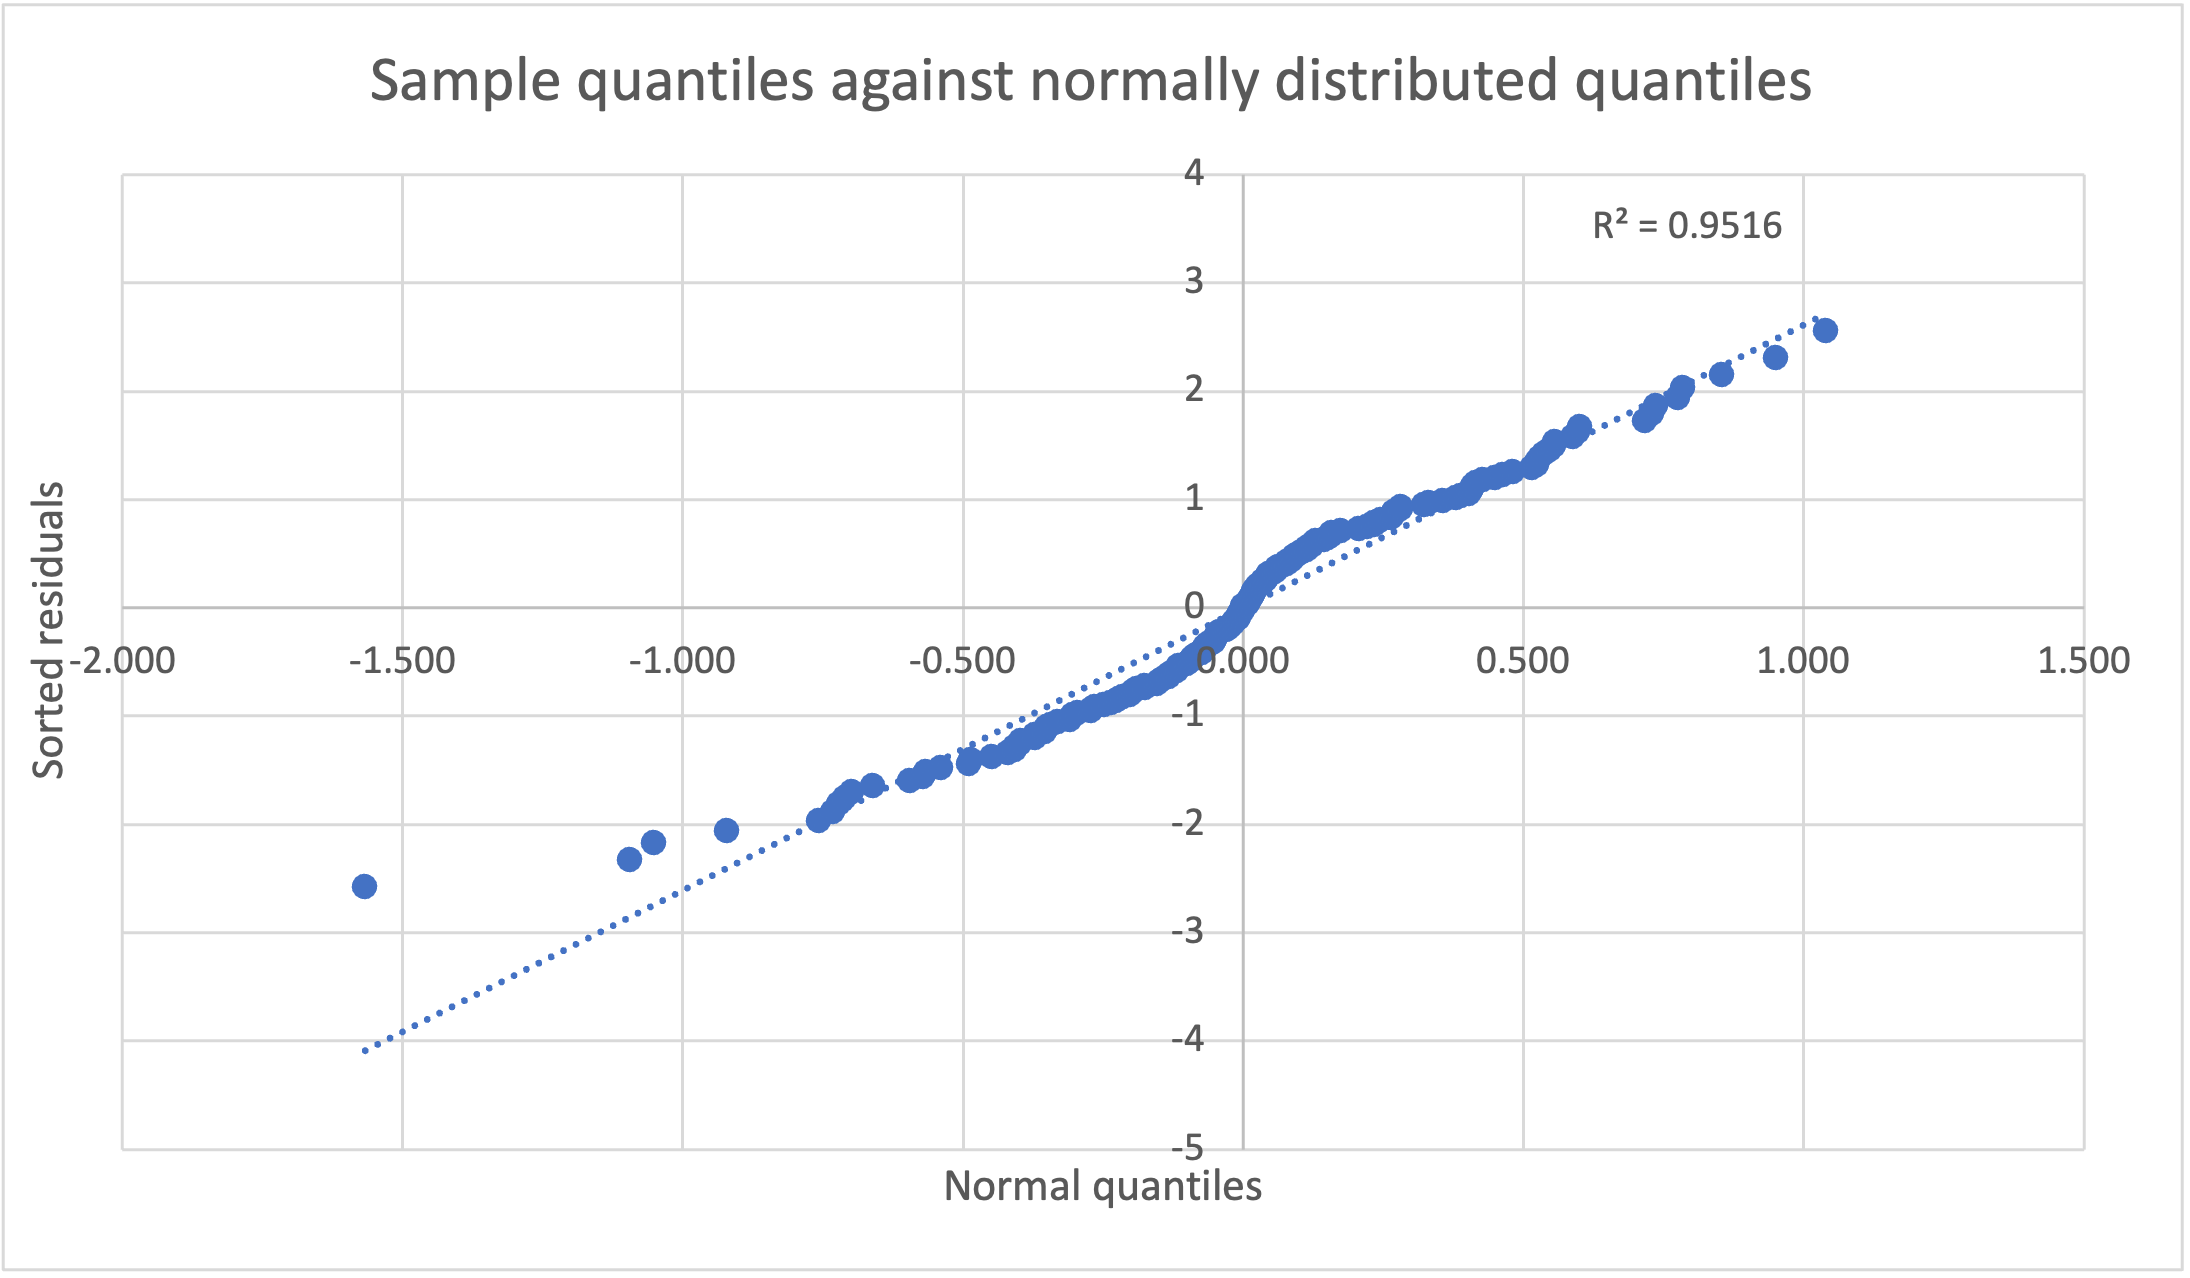
\includegraphics[width=0.85\textwidth]{Images/QQplot.png}
    \caption{QQ Plot of Model Residuals}
    \label{fig:qqplotresid}
\end{figure}

\begin{figure}[H]
     \centering
     \begin{subfigure}[b]{0.475\textwidth}
         \centering
         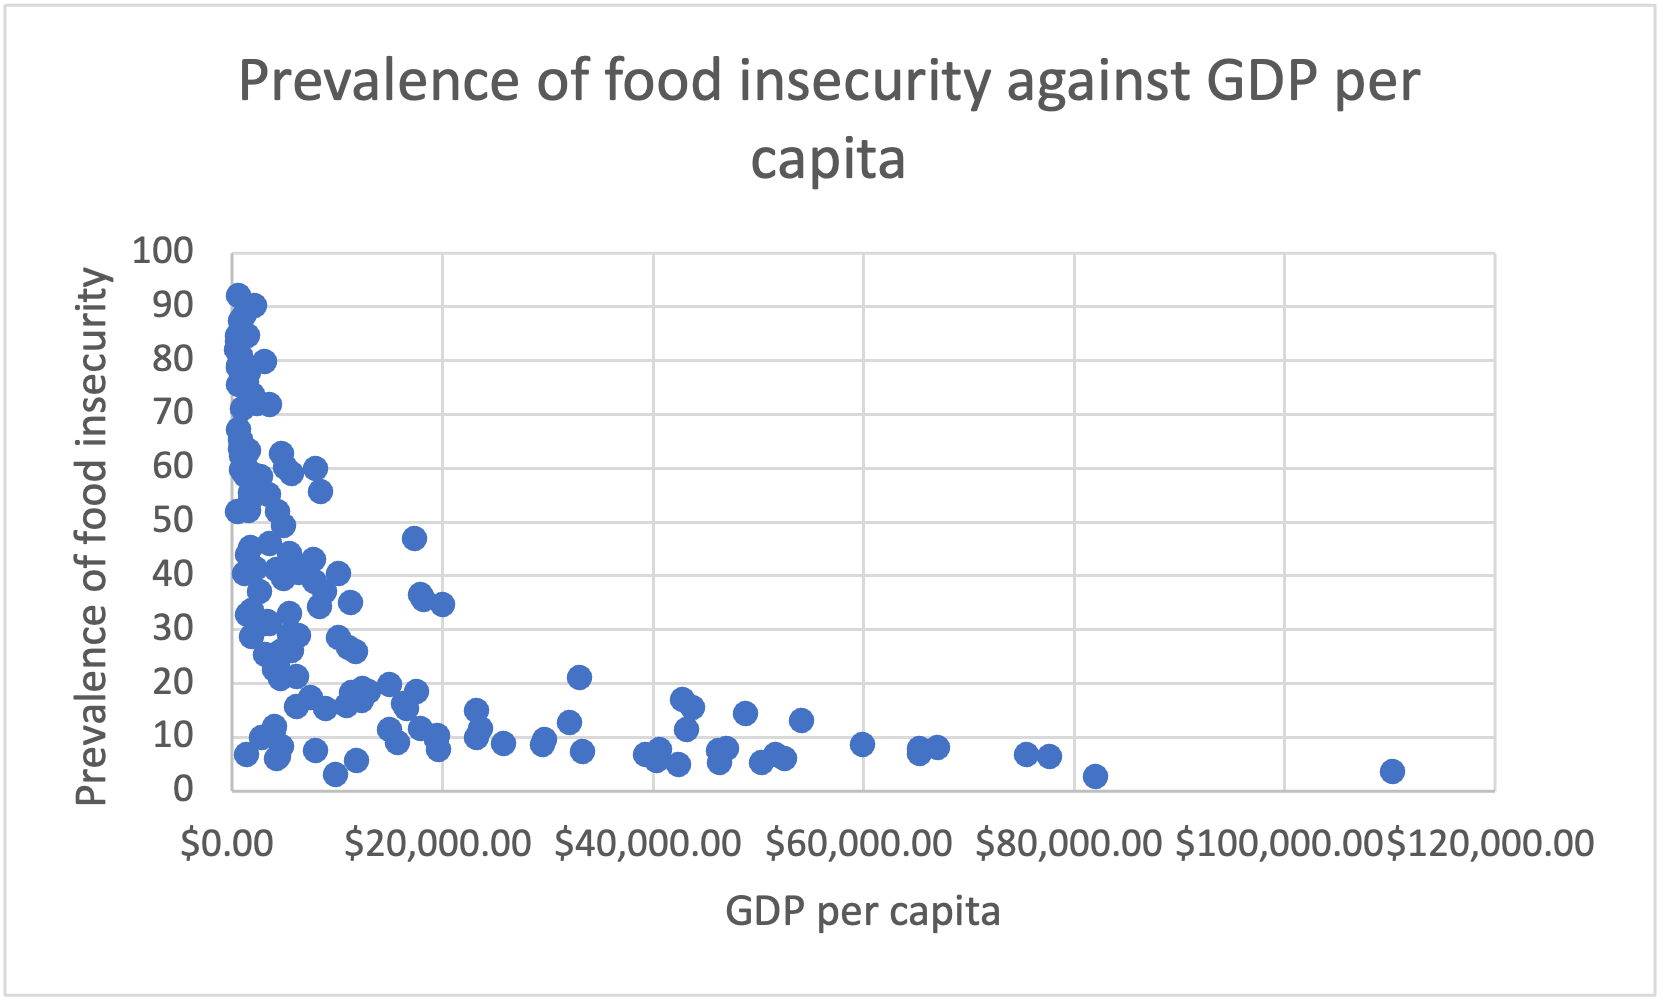
\includegraphics[width=\textwidth]{Images/gdppc.png}
         \caption{FII vs. GDPpc}
         \label{fig:gdppcscatter}
     \end{subfigure}
     \hfill
     \begin{subfigure}[b]{0.475\textwidth}
         \centering
         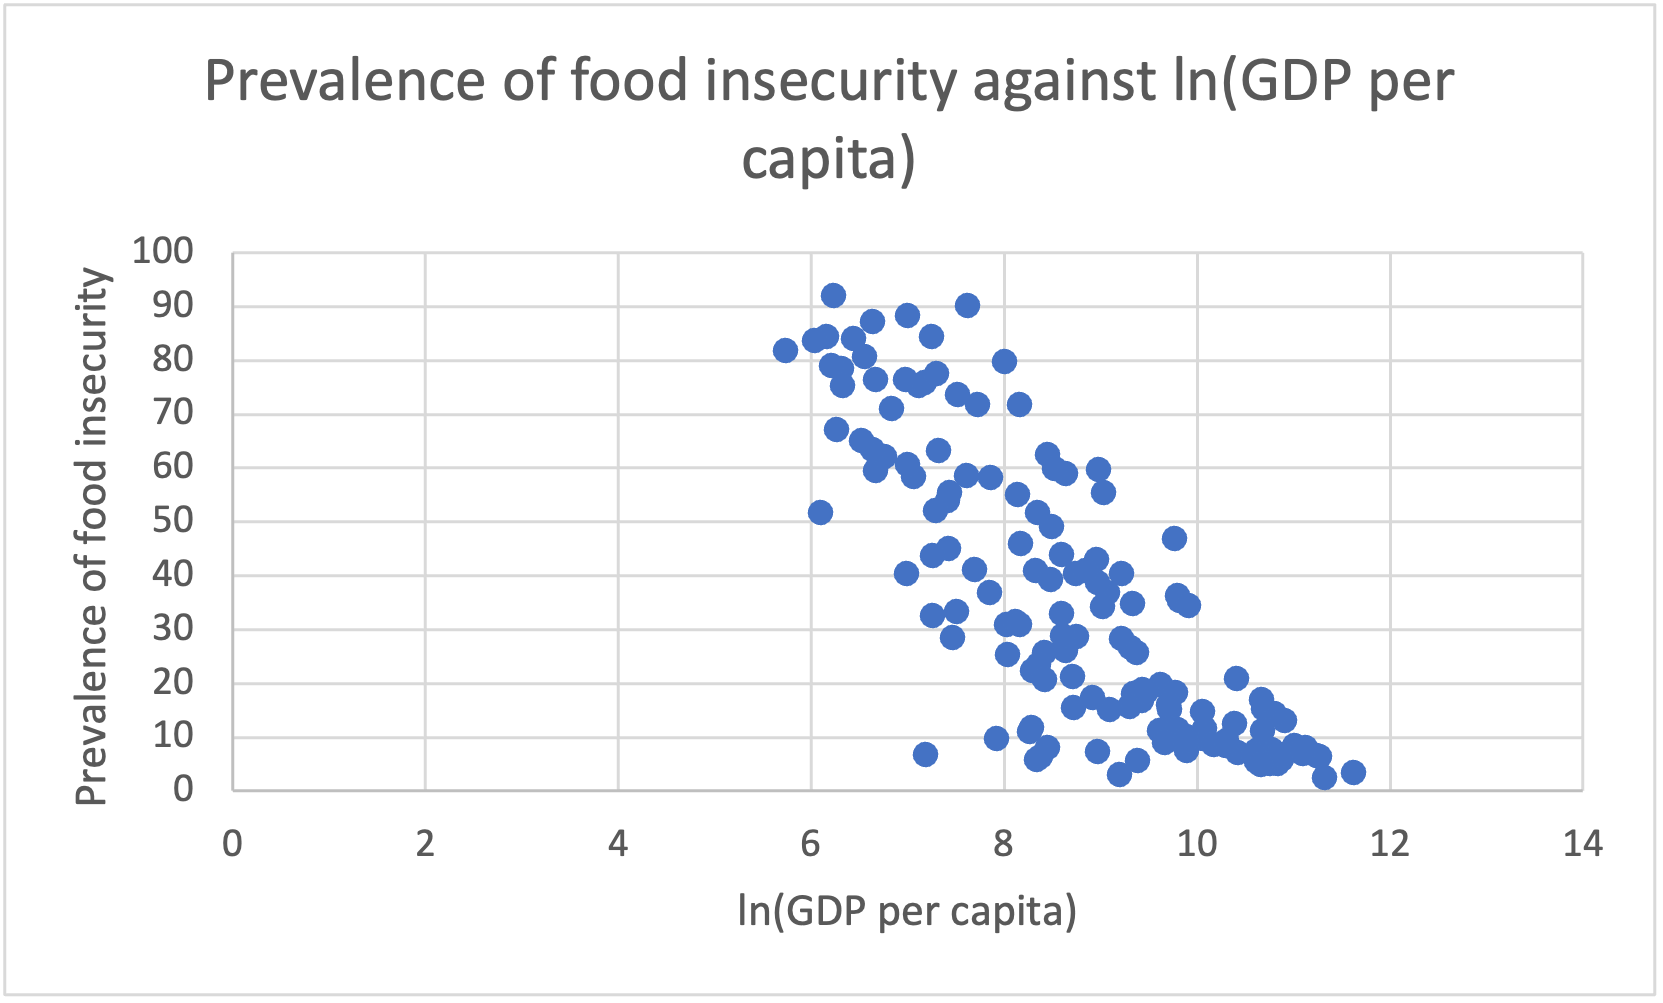
\includegraphics[width=\textwidth]{Images/lngdppc.png}
         \caption{FII vs. $\ln{[\text{GDPpc}]}$}
         \label{fig:lggpdpcscatter}
     \end{subfigure}
    \caption{Scatter Plots of FII against GDPpc}
    \label{fig:scattergdppc}
\end{figure}

\begin{figure}[H]
     \centering
     \begin{subfigure}[b]{0.475\textwidth}
         \centering
         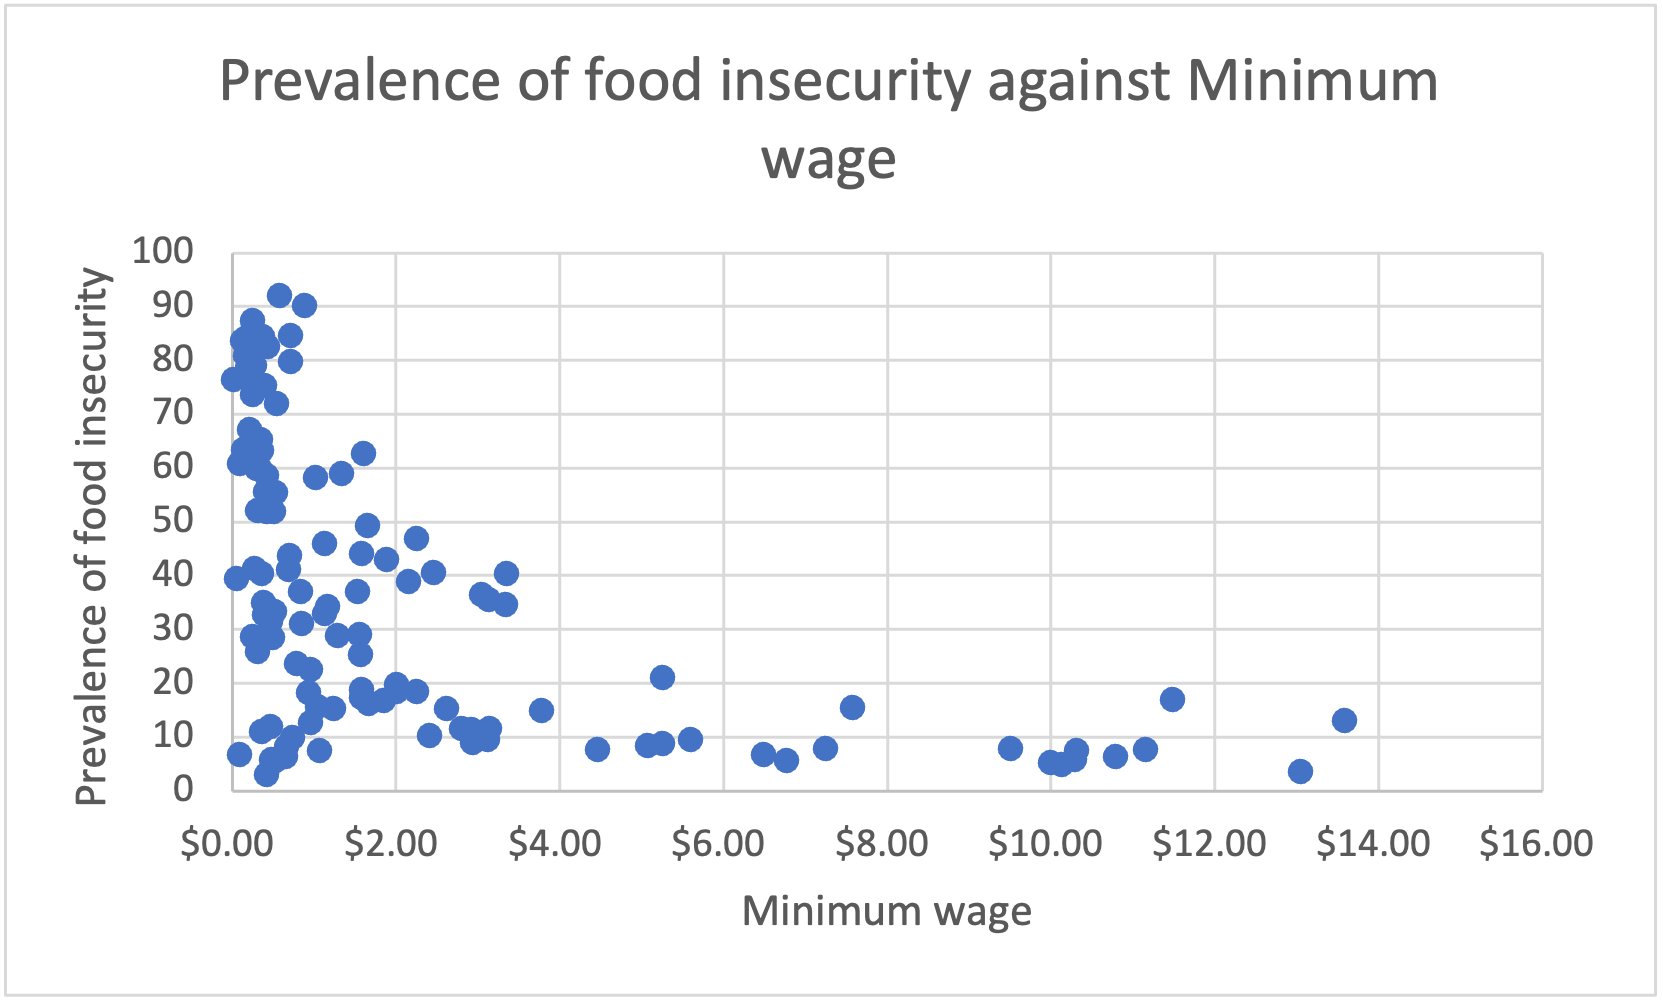
\includegraphics[width=\textwidth]{Images/minwage.png}
         \caption{FII vs. MinimumWage}
         \label{fig:ffiminwagescatter}
     \end{subfigure}
     \hfill
     \begin{subfigure}[b]{0.475\textwidth}
         \centering
         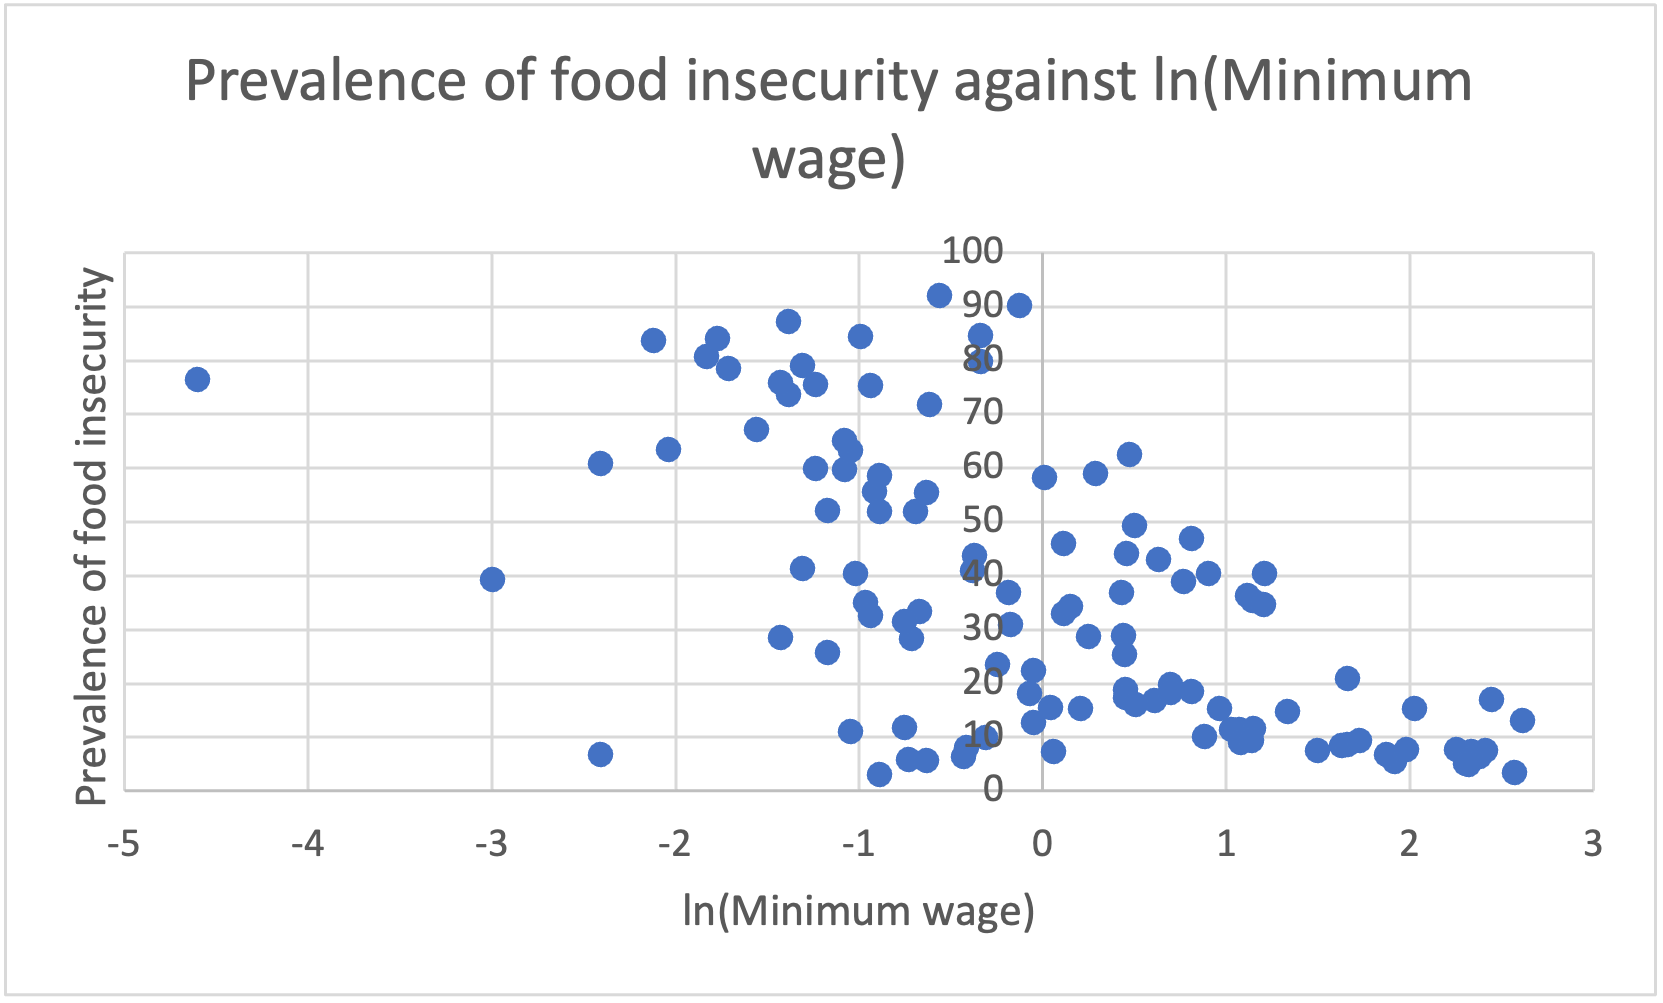
\includegraphics[width=\textwidth]{Images/lnminwage.png}
         \caption{FII vs. $\ln{[\text{MinimumWage}]}$}
         \label{fig:ffilnminwagescatter}
     \end{subfigure}
    \caption{Scatter Plots of FII against Minimum Wage}
    \label{fig:scatterminwage}
\end{figure}

\begin{figure}[H]
     \centering
     \begin{subfigure}[b]{0.475\textwidth}
         \centering
         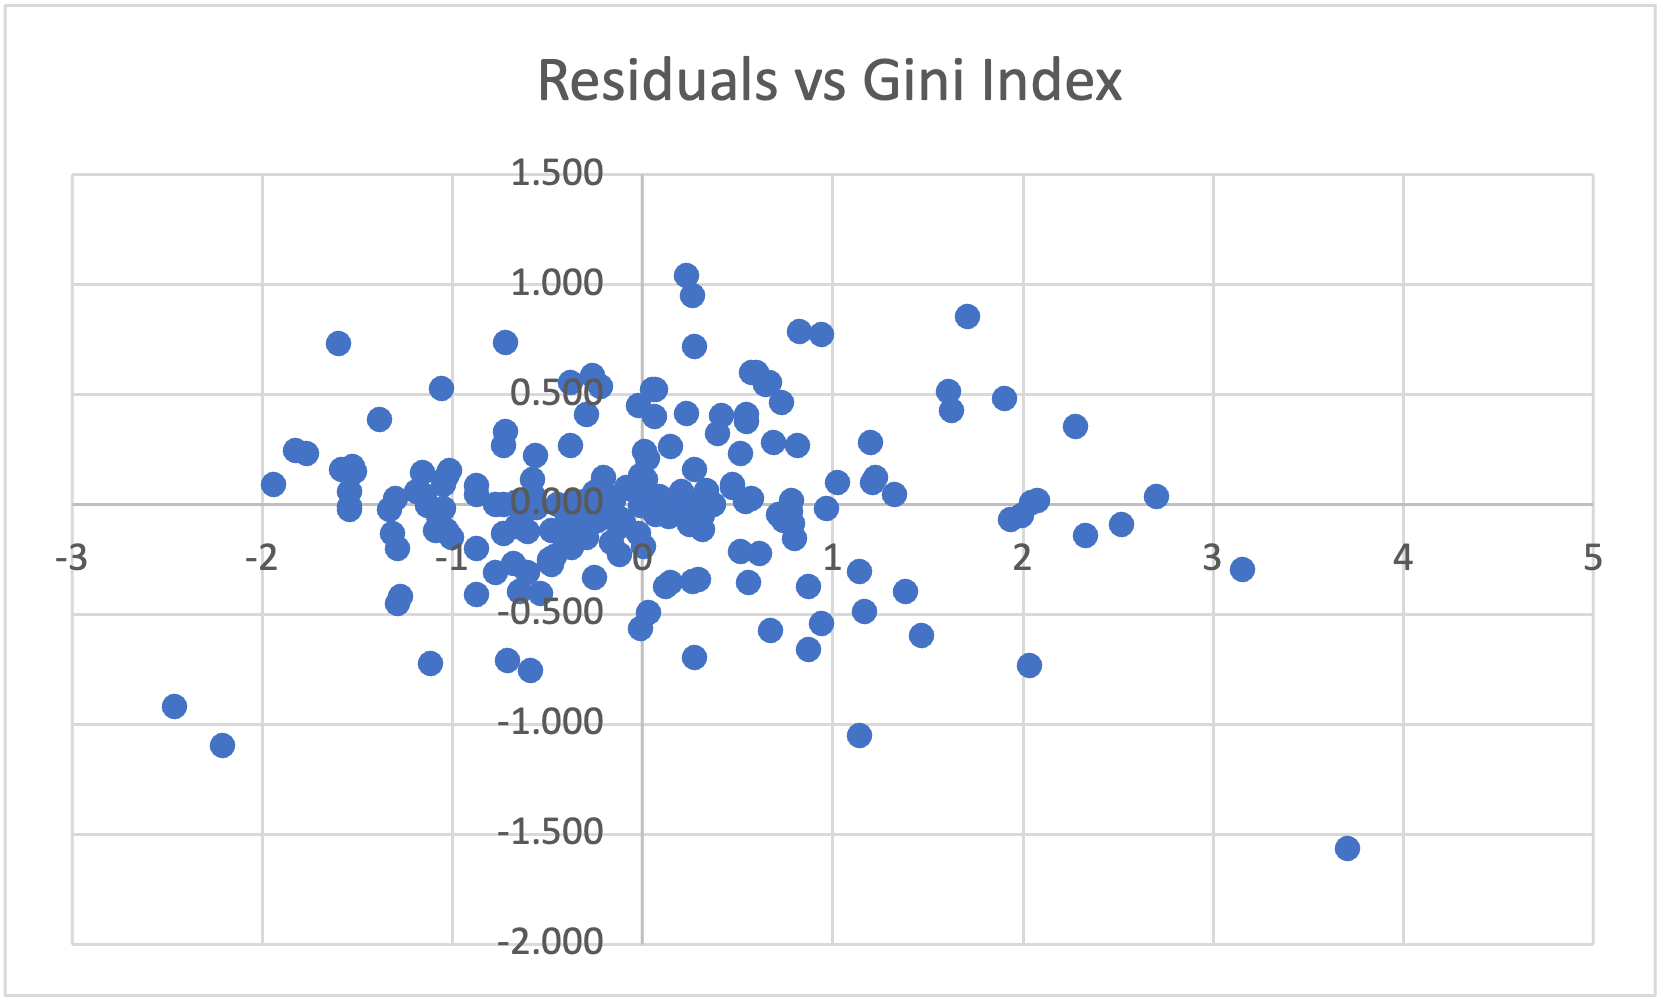
\includegraphics[width=\textwidth]{Images/resgini.png}
         \caption{Residuals vs. GiniIndex}
         \label{fig:resgini}
     \end{subfigure}
     \hfill
     \begin{subfigure}[b]{0.475\textwidth}
         \centering
         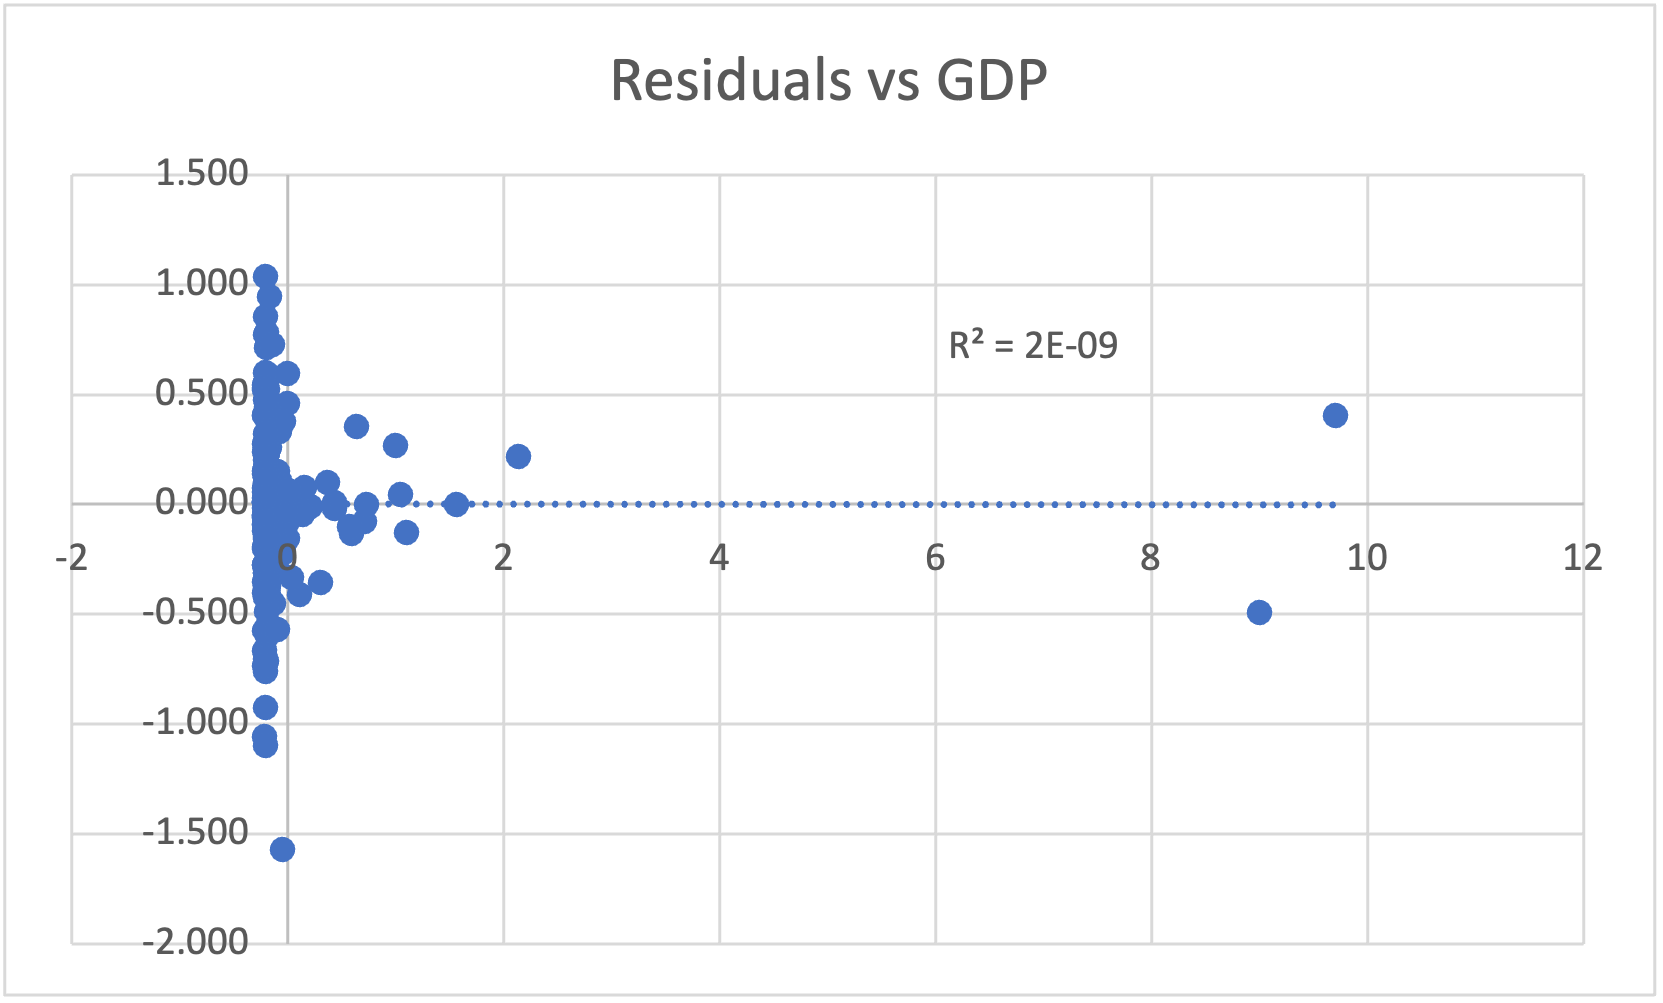
\includegraphics[width=\textwidth]{Images/resgdp.png}
         \caption{Residuals vs. GDP}
         \label{fig:resgdp}
     \end{subfigure}
    \caption{Residuals vs. GDP}
    \label{fig:scatterresid1}
\end{figure}

\begin{figure}[H]
     \centering
     \begin{subfigure}[b]{0.475\textwidth}
         \centering
         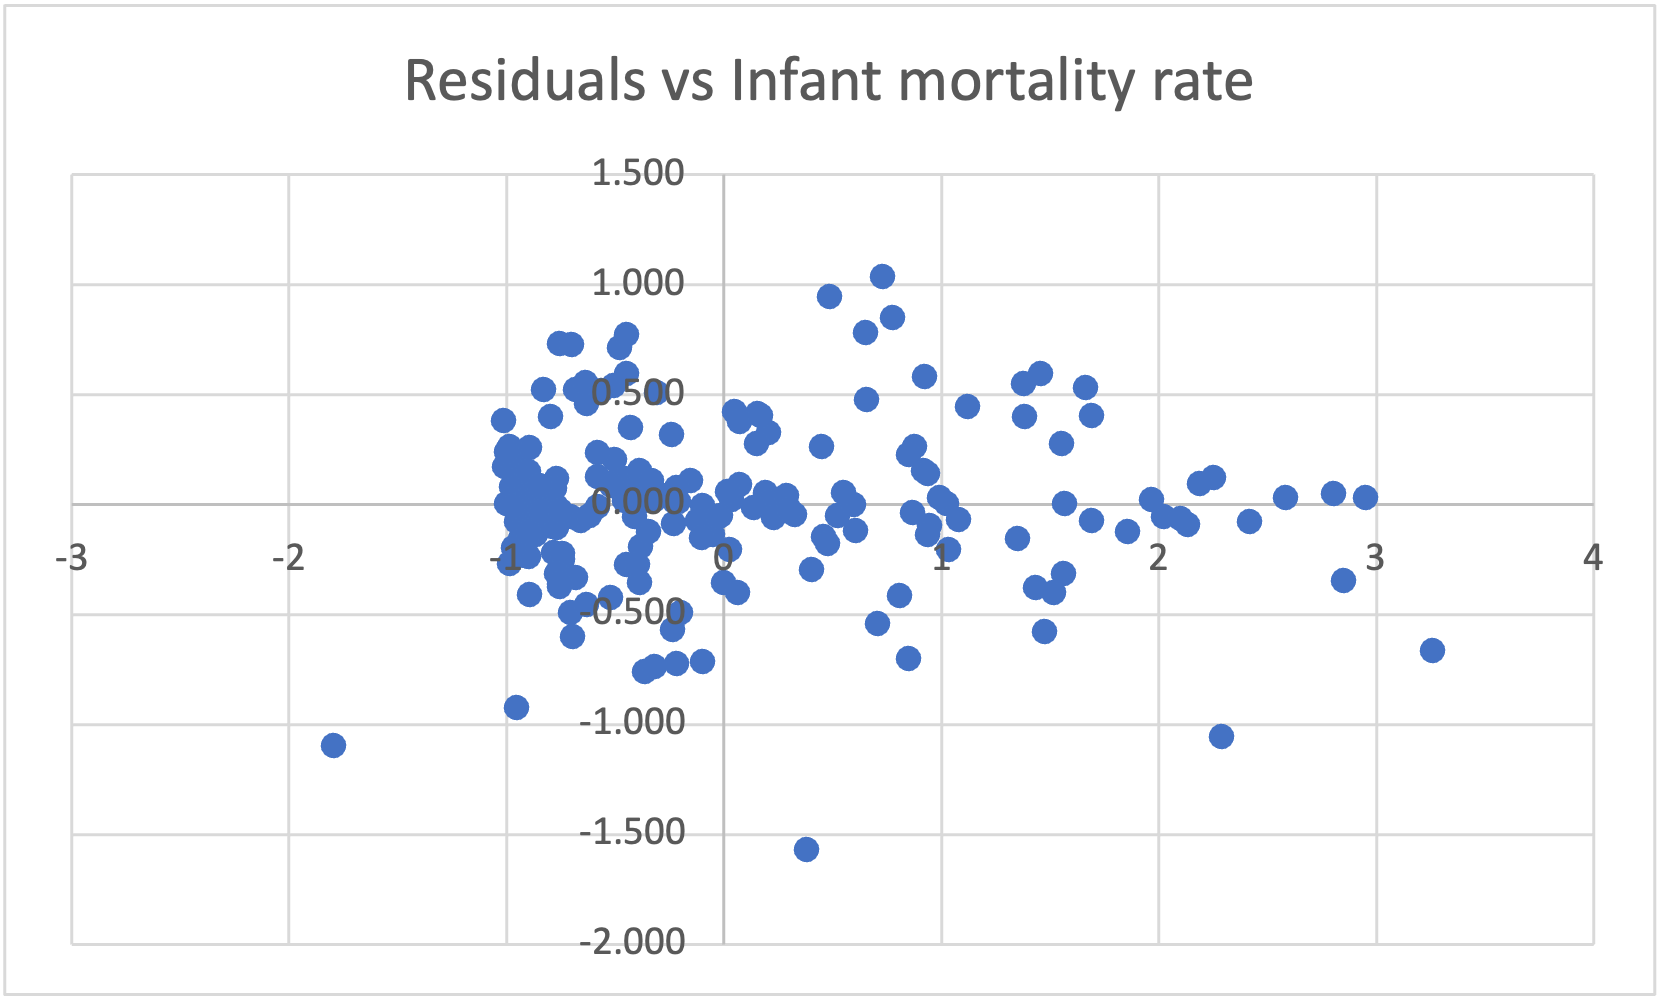
\includegraphics[width=\textwidth]{Images/resinf.png}
         \caption{Residuals vs. InfantMortality}
         \label{fig:resinf}
     \end{subfigure}
     \hfill
     \begin{subfigure}[b]{0.475\textwidth}
         \centering
         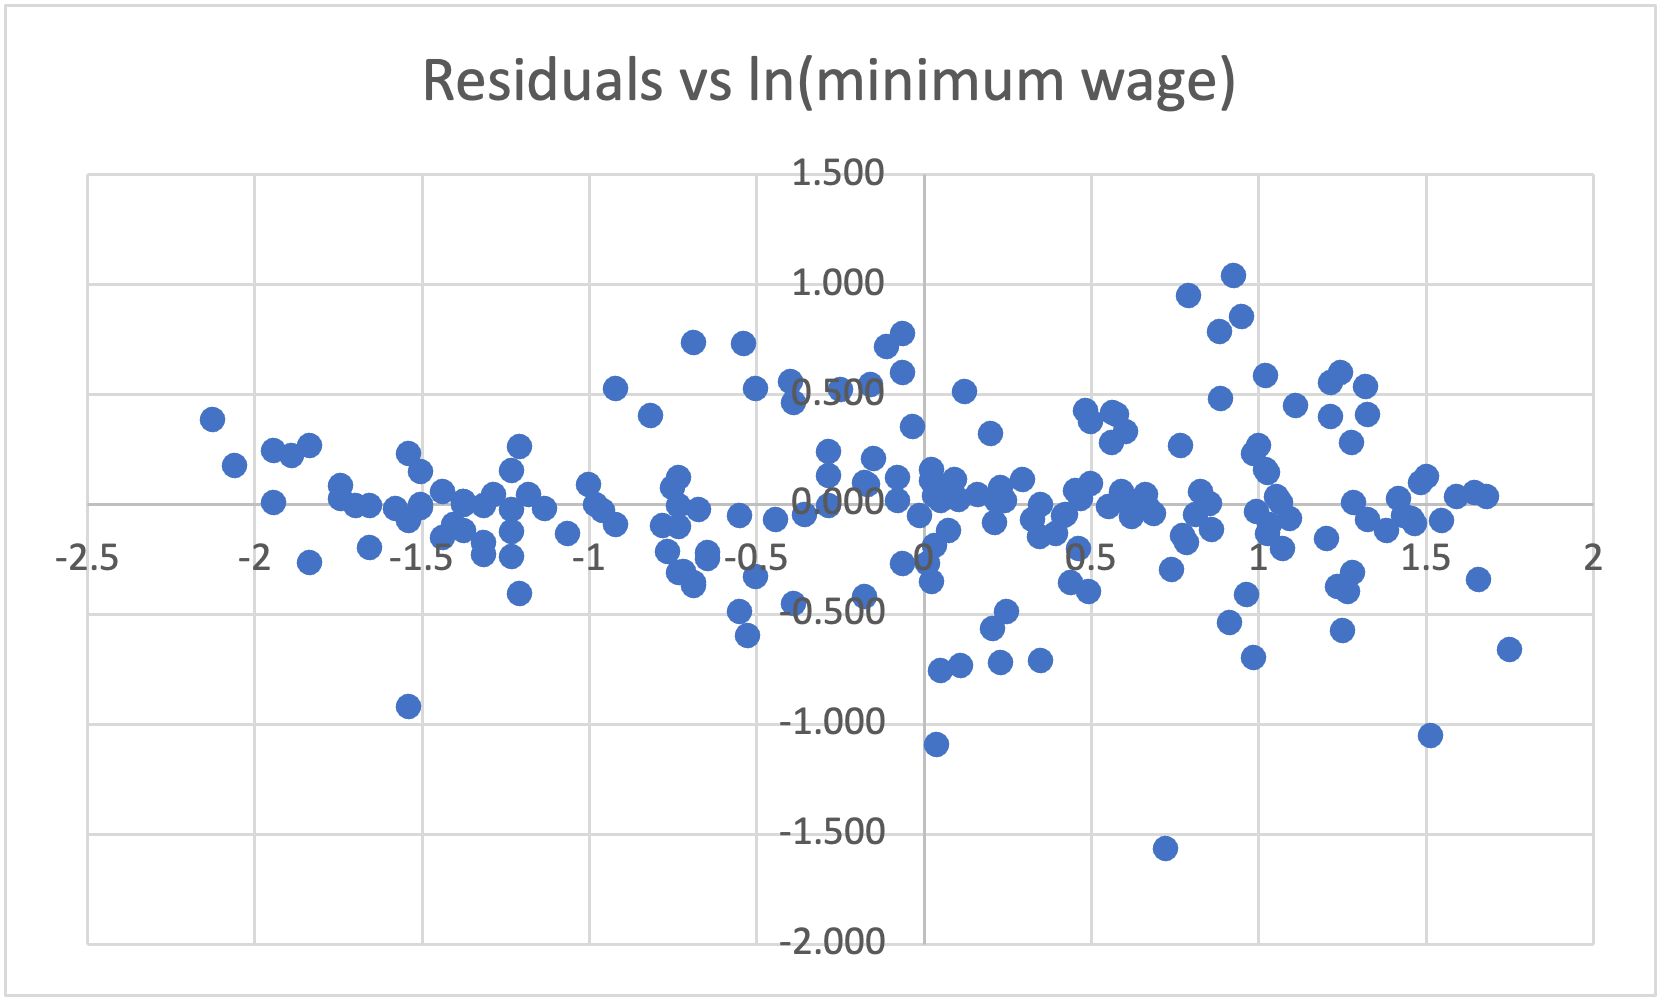
\includegraphics[width=\textwidth]{Images/resminwage.png}
         \caption{Residuals vs. MinimumWage}
         \label{fig:resminwage}
     \end{subfigure}
    \caption{Scatter Plots of Residuals against Predictors}
    \label{fig:scatterresid2}
\end{figure}

\begin{figure}[H]
    \centering
    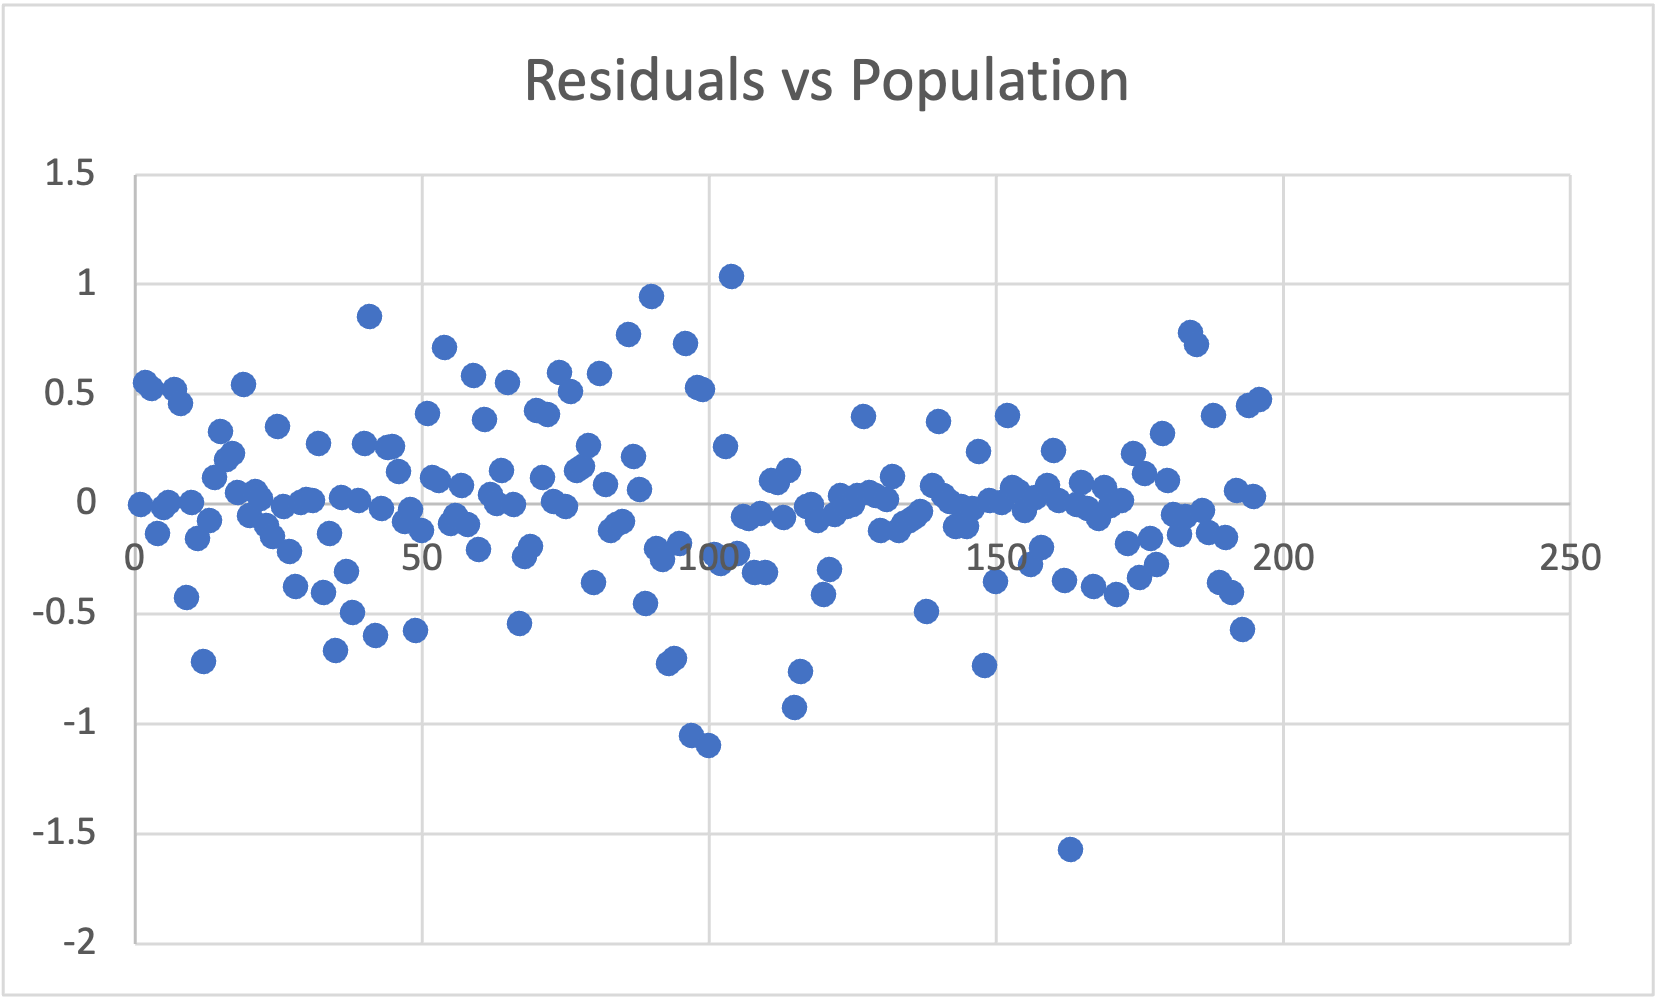
\includegraphics[width=0.5\textwidth]{Images/respop.png}
    \caption{Scatter Plots of Residuals against Population}
    \label{fig:scatterresid3}
\end{figure}

\begin{figure}[H]
    \centering
    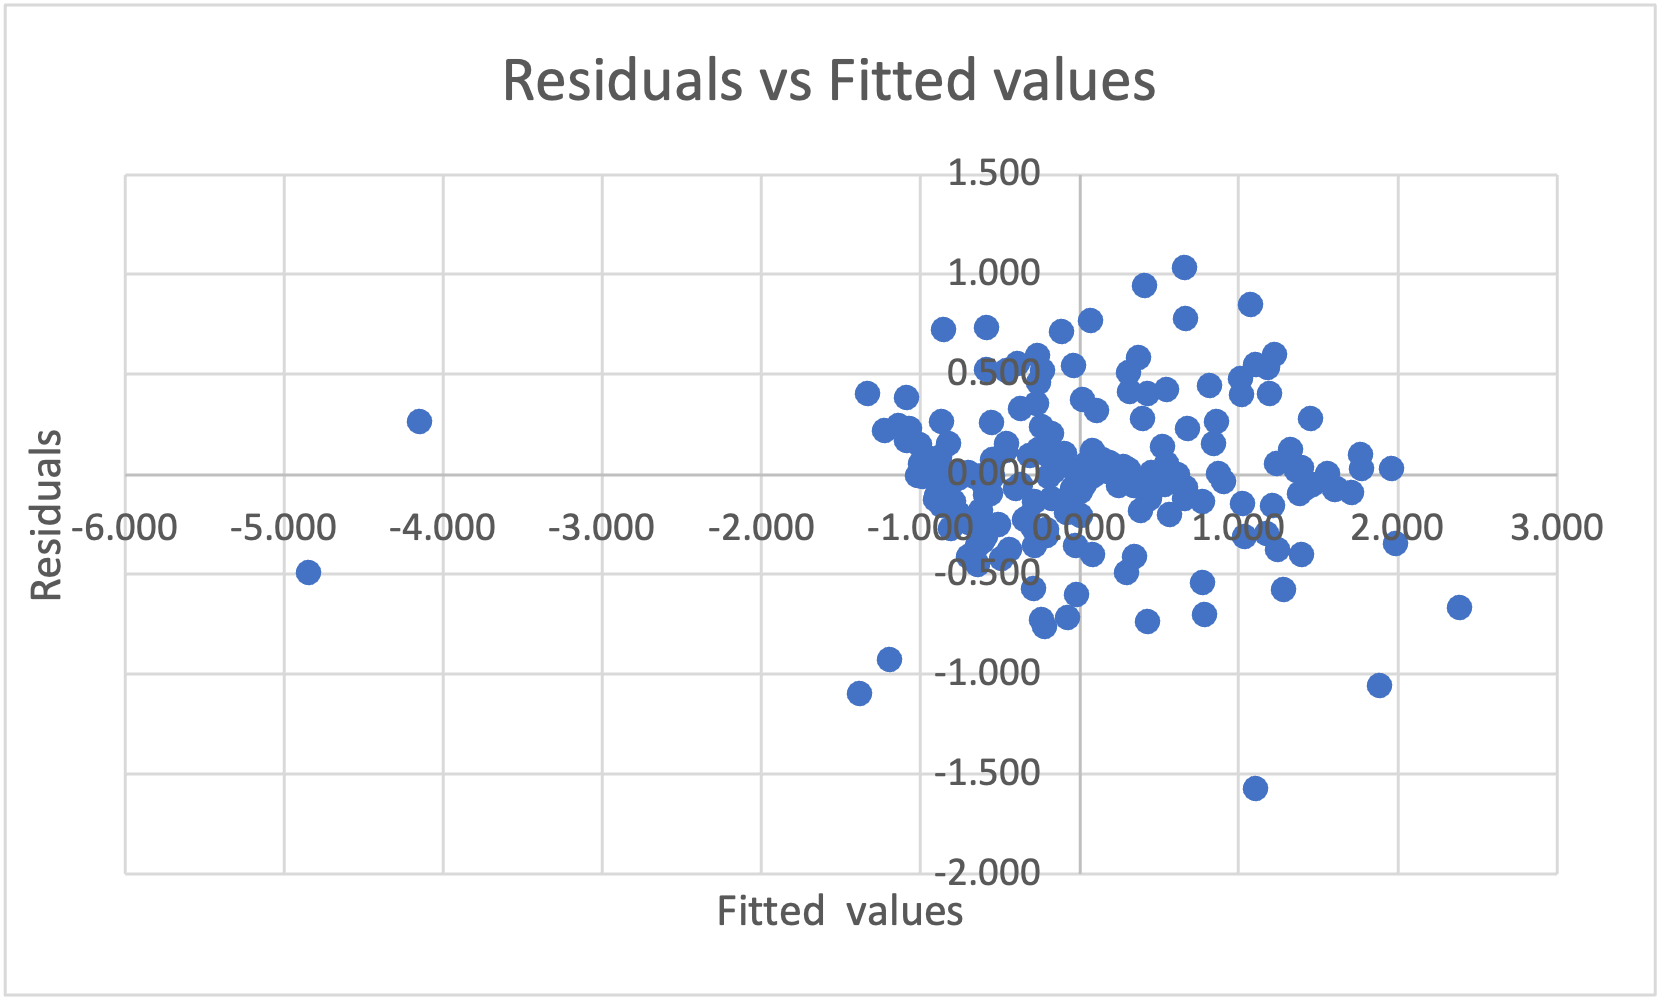
\includegraphics[width=0.85\textwidth]{Images/resfit.png}
    \caption{Scatter Plots of Residuals against Fitted Values of Model}
    \label{fig:scatterresfit}
\end{figure}

\section{OLS Parameter Estimates for Each Model}\label{AppB}

\begin{table}[H]
    \centering
        \begin{threeparttable}
            \begin{tabular}{l l l l l}
              \toprule & \textbf{Estimate} & \textbf{Std. Error} & \textbf{t-statistic} & \textbf{p-value} \\ \midrule
            \textbf{$\beta_0$} & 0.000 & 0.024 & 0.000 & 1.000 \\ 
            \textbf{$\beta_1$ AgriculturalLand(\%)} & -0.017 & 0.027 & -0.620 & 0.536  \\ 
            \textbf{$\beta_2$ $\bm{CO_2}$Emissions} & -0.193 & 0.097 & -1.996 & 0.047 $**$  \\ 
            \textbf{$\beta_3$ CPI} & 0.004 & 0.026 & 0.150 & 0.881 \\ 
            \textbf{$\beta_4$ GDP} & 0.190 & 0.071 & 2.662 & 0.008 $***$ \\ 
            \textbf{$\beta_5$ Population} & -0.431 & 0.049 & -8.818 & $\num{1.00e-04}$ $***$ \\ 
            \textbf{$\beta_6$ InfantMortality} & 0.418 & 0.059 & 7.118 & $\num{1.00e-04}$ $***$ \\ 
            \textbf{$\beta_7$ $\bm{\ln{[\text{MinimumWage}]}}$} & -0.079 & 0.067 & -1.177 & 0.241 \\ 
            \textbf{$\beta_8$ Unemployment(\%)} & -0.029 & 0.032 & -0.896 & 0.371 \\ 
            \textbf{$\beta_9$ LabourForceParticipation} & -0.045 & 0.030 & -1.516 & 0.131 \\ 
            \textbf{$\beta_{10}$ Temperature} & 0.069 & 0.044 & 1.571 & 0.118 \\ 
            \textbf{$\beta_{11}$ IdealTemperature} & 0.051 & 0.033 & 1.546 & 0.124 \\ 
            \textbf{$\beta_{12}$ PrecipitationDepth} & -0.013 & 0.027 & -0.490 & 0.625 \\ 
            \textbf{$\beta_{13}$ GiniIndex} & 0.193 & 0.034 & 5.601 & $\num{1.00e-04}$ $***$\\ 
            \textbf{$\beta_{14}$ $\bm{\ln{[\text{GDPpc}]}}$} & -0.017 & 0.044 & -0.381 & 0.704 \\ 
            \textbf{$\beta_{15}$ HDI} & -0.351 & 0.078 & -4.493 & $\num{1.00e-04}$ $***$ \\ \bottomrule
            \end{tabular}
            \begin{tablenotes}
                \small
                \item *** $p < 0.01$, ** $p < 0.05$, * $p < 0.1$
            \end{tablenotes}
        \end{threeparttable}
    \caption{\label{table: descriptivestatsoriginal}\textbf{Original} Multiple Linear Regression Model Parameter Estimates}
\end{table}

\begin{table}[H]
    \centering
        \begin{threeparttable}
            \begin{tabular}{l l l l l}
              \toprule & \textbf{Estimate} & \textbf{Std. Error} & \textbf{t-statistic} & \textbf{p-value} \\ \midrule
            \textbf{$\beta_0$} & 0.000 & 0.043 & 0.000 & 1.000 \\ 
            \textbf{$\beta_1$ CPI} & 0.044 & 0.044 & 1.009 & 0.314  \\ 
            \textbf{$\beta_2$ $\bm{\ln{[\text{MinimumWage}]}}$} & 0.572 & 0.049 & 11.593 & $\num{1.00e-04}$ $***$  \\ 
            \textbf{$\beta_3$ Unemployment(\%)} & -0.007 & 0.054 & -0.125 & 0.901 \\ 
            \textbf{$\beta_4$ LabourForceParticipation} & 0.017 & 0.052 & 0.338 & 0.736 \\ 
            \textbf{$\beta_5$ GiniIndex} & 0.222 & 0.054 & 4.107 & $\num{1.00e-04}$ $***$ \\ 
            \textbf{$\beta_6$ GDP} & -0.301 & 0.043 & -6.940 & $\num{1.00e-04}$ $***$ \\ \bottomrule
            \end{tabular}
            \begin{tablenotes}
                \small
                \item *** $p < 0.01$, ** $p < 0.05$, * $p < 0.1$
            \end{tablenotes}
        \end{threeparttable}
    \caption{\label{table: descriptivestatseconomic}\textbf{Economic} Multiple Linear Regression Model Parameter Estimates}
\end{table}

\begin{table}[H]
    \centering
        \begin{threeparttable}
            \begin{tabular}{l l l l l}
              \toprule & \textbf{Estimate} & \textbf{Std. Error} & \textbf{t-statistic} & \textbf{p-value} \\ \midrule
            \textbf{$\beta_0$} & 0.000 & 0.027 & 0.000 & 1.000 \\ 
            \textbf{$\beta_1$ AgriculturalLand(\%)} & 0.000 & 0.029 & 0.011 & 0.991  \\ 
            \textbf{$\beta_2$ $\bm{\text{CO}_2}$Emissions} & 0.047 & 0.047 & 1.004 & 0.317 \\ 
            \textbf{$\beta_3$ Population} & -0.517 & 0.047 & -11.012 & $\num{1.00e-04}$ $***$ \\ 
            \textbf{$\beta_4$ InfantMortalityRate} & 0.394 & 0.057 & 6.974 & $\num{1.00e-04}$ $***$ \\ 
            \textbf{$\beta_5$ IdealTemperature} & 0.120 & 0.029 & 4.1032 & $\num{1.00e-04}$ $***$ \\ 
            \textbf{$\beta_6$ PrecipitationDepth} & -0.020 & 0.029 & 0.692 & 0.490 \\ 
            \textbf{$\beta_7$ HDI} & -0.409 & 0.058 & -7.064 & $\num{1.00e-04}$ $***$ \\ \bottomrule
            \end{tabular}
            \begin{tablenotes}
                \small
                \item *** $p < 0.01$, ** $p < 0.05$, * $p < 0.1$
            \end{tablenotes}
        \end{threeparttable}
    \caption{\label{table: descriptivestatsgeographic}\textbf{Geographic} Multiple Linear Regression Model Parameter Estimates}
\end{table}

\begin{table}[H]
    \centering
        \begin{threeparttable}
            \begin{tabular}{l l l l l}
              \toprule & \textbf{Estimate} & \textbf{Std. Error} & \textbf{t-statistic} & \textbf{p-value} \\ \midrule
            \textbf{$\beta_0$} & 0.000 & 0.027 & 0.000 & 1.000 \\ 
            \textbf{$\beta_1$ GDP} & 0.006 & 0.035 & 0.176 & 0.860  \\ 
            \textbf{$\beta_2$ Population} & -0.476 & 0.035 & -13.676 & $\num{1.00e-04}$ $***$ \\ 
            \textbf{$\beta_3$ InfantMortality} & 0.560 & 0.059 & 9.576 & $\num{1.00e-04}$ $***$ \\ 
            \textbf{$\beta_4$ $\bm{\ln{[\text{MinimumWage}]}}$} & 0.145 & 0.062 & 2.333 & 0.021 $**$ \\ 
            \textbf{$\beta_5$ GiniIndex} & 0.229 & 0.030 & 7.582 & $\num{1.00e-04}$ $***$ \\ \bottomrule
            \end{tabular}
            \begin{tablenotes}
                \small
                \item *** $p < 0.01$, ** $p < 0.05$, * $p < 0.1$
            \end{tablenotes}
        \end{threeparttable}
    \caption{\label{table: descriptivestatsfinal}\textbf{Final} Multiple Linear Regression Model Parameter Estimates}
\end{table}

\section{Inferential Statistics of Models}\label{AppC}
\begin{table}[H]
    \centering
        \begin{threeparttable}
            \begin{tabular}{l l l l l}
              \toprule \textbf{Model Type} & \textbf{Adjusted $\bm{R^2}$} & \textbf{F-Statistic} & \textbf{AIC} & \textbf{BIC} \\ \midrule
            \textbf{Original Model} & 0.889 & 104.749 & -413.626 & -361.258 \\ 
            \textbf{Economic Model} & 0.647 & 60.272 & -196.199 & -173.288  \\ 
            \textbf{Geographical Model} & 0.861 & 172.132 & -376.433 & -350.249 \\ 
            \textbf{Final Model} & 0.862 & 244.069 & -380.784 & -361.146 \\ \bottomrule
            \end{tabular}
        \end{threeparttable}
    \caption{\label{table: infstatsallmodel}Inferential Statistics of All Models}
\end{table}

\section{Correlation Matrix of Final Model}\label{AppE}

\begin{table}[H]
    \centering
        \begin{threeparttable}
            \begin{tabular}{l l l l l l l}
              \toprule & \textbf{GDP} & \textbf{Population} & \textbf{InfantMortality} & \textbf{$\bm{\ln{[\text{MinWage}]}}$} & \textbf{GiniIndex} & \textbf{FII} \\ \midrule 
            \textbf{GDP} & $\bm{1}$ & 0.625 & -0.150 & -0.170 & -0.011 & -0.403 \\ 
            \textbf{Population} & $\bm{\textcolor{red}{0.625}}$ & $\bm{1}$ & 0.006 & 0.027 & 0.008 & -0.463 \\ 
            \textbf{InfantMortality} & -0.150 & 0.006 & $\bm{1}$ & 0.888 & 0.352 & 0.766 \\ 
            \textbf{$\bm{\ln{[\text{MinWage}]}}$} & -0.170 & 0.027 & $\bm{\textcolor{red}{0.888}}$ & $\bm{1}$ & 0.453 & 0.733 \\ 
            \textbf{GiniIndex} & -0.011 & 0.008 & $\bm{\textcolor{red}{0.352}}$ & $\bm{\textcolor{red}{0.453}}$ & $\bm{1}$ & 0.489\\ 
            \textbf{FII} & -0.403 & -0.463 & 0.766 & 0.733 & 0.489 & $\bm{1}$ \\ \bottomrule
            \end{tabular}
        \end{threeparttable}
    \caption{\label{table: corrmatrix}\textbf{Final} Multiple Linear Regression Model Correlation Matrix \textbf{(Mirrored along Diagonal)}}
\end{table}

\end{appendices}

\newpage
\bibliographystyle{plain}
\bibliography{refs}

\end{document}
